\section{Results and analysis}
\label{sec:results}

\subsection{Clean baseline and the main degradation grid}
\label{sec:results:main}

Table~\ref{tab:main} reports sentence-level error rates on the main grid for
the five recognition systems, and Fig.~\ref{fig:heatmap} visualises the same
data split by language. On clean synthetic speech the three foundation-model
recognisers are close to their scoring floor, with error rates between 0.3
and 0.5 percent, while the specialised streaming recogniser operates at 0.56
percent on Chinese and 3.99 percent on English, reflecting its primarily
Mandarin training. The telephone-band specialist reaches 1.86 percent on its
native language. The clean-condition figures establish that the comparisons
under degradation are not confounded by differences in clean accuracy of
comparable magnitude.

\begin{table}[t]
\centering
\caption{Mean recognition error rates in percent on the main degradation
grid, both languages pooled, with bootstrap 95 percent confidence intervals
in parentheses. The 8~kHz specialist is evaluated on the Chinese subset only.}
\label{tab:main}
\footnotesize
\setlength{\tabcolsep}{2.6pt}
\begin{tabular}{lccccccccc}
\toprule
System & Clean & Babble 10 & Babble 0 & Reverb & Narrow & Codec & Loss & Clip & Tempo \\
\midrule
Paraformer-v2 & 2.3 & 2.8 & 58.5 & 3.2 & 2.1 & 2.4 & 3.2 & 2.5 & 2.3 \\
 & (2,3) & (2,4) & (54,63) & (2,4) & (2,3) & (2,3) & (2,4) & (2,3) & (2,3) \\
Paraformer-8K & 1.9 & 4.7 & 73.2 & 18.2 & 1.9 & 1.8 & 3.3 & 1.9 & 2.3 \\
 & (1,3) & (3,6) & (69,78) & (14,22) & (1,3) & (1,3) & (2,5) & (1,3) & (2,3) \\
Qwen-Audio-3.1 & 0.5 & 0.9 & 28.2 & 0.7 & 0.6 & 0.6 & 0.6 & 0.9 & 0.6 \\
 & (0,1) & (1,1) & (25,32) & (0,1) & (0,1) & (0,1) & (0,1) & (1,1) & (0,1) \\
Qwen3-ASR & 0.3 & 0.5 & 25.1 & 0.3 & 0.3 & 0.3 & 0.4 & 0.3 & 0.3 \\
 & (0,0) & (0,1) & (22,29) & (0,0) & (0,0) & (0,0) & (0,1) & (0,0) & (0,0) \\
Qwen3.8-Omni & 0.4 & 0.6 & 31.8 & 1.1 & 0.1 & 0.3 & 0.2 & 1.0 & 0.3 \\
 & (0,1) & (0,1) & (28,36) & (1,2) & (0,0) & (0,0) & (0,0) & (1,2) & (0,0) \\
\bottomrule
\end{tabular}
\end{table}

\begin{figure}[t]
\centering
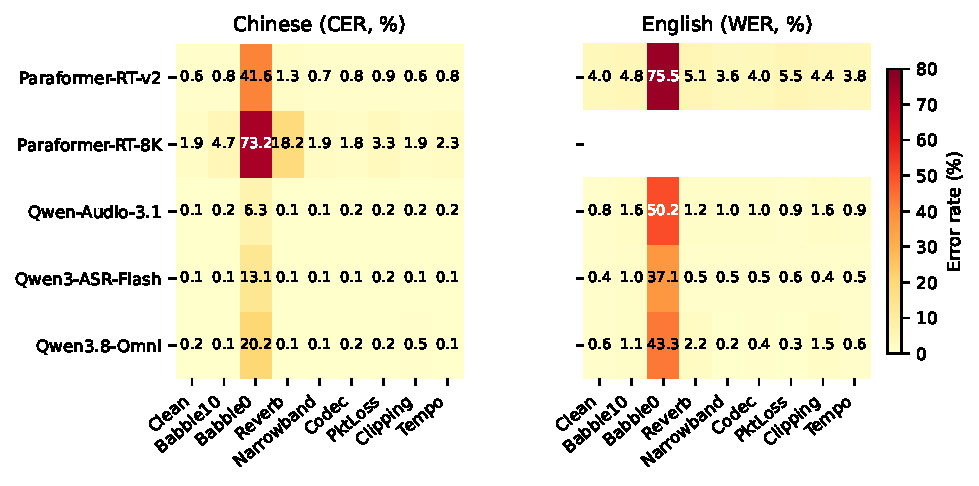
\includegraphics[width=\textwidth]{../figures/fig2_heatmap.pdf}
\caption{Recognition error rates by system and degradation condition,
separated by language. Colour scale is truncated at 80 percent. The 8~kHz
specialist is evaluated on the Chinese subset only.}
\label{fig:heatmap}
\end{figure}

Three regularities stand out in the grid. First, babble noise at 0~dB is by
far the most destructive condition for every system, but the magnitude of
the collapse separates the product classes sharply. The specialised
streaming recogniser reaches a pooled error rate of 58.5 percent and the
telephone-band specialist 73.2 percent, whereas the two LLM-ASR systems
remain at 25 to 28 percent and the omni model at 31.8 percent. At matched
severity, the foundation-model recognisers commit roughly half the error of
the specialised systems, and the difference is significant at the sentence
level: in Chinese at 0~dB, Qwen-Audio 3.1 errs at 6.3 percent against 41.6
percent for the streaming specialist (Wilcoxon $p<0.001$, $n=240$).

Second, the effect of noise is strongly language-asymmetric in a way that
differs by class. For the LLM-ASR systems, Chinese recognition at 0~dB
remains low, at 6.3 percent for Qwen-Audio 3.1 and 13.1 percent for Qwen3
ASR, while their English error rates at the same severity reach 50.2 and 37.1
percent. The specialised streaming recogniser suffers heavily in both
languages, 41.6 percent in Chinese and 75.5 percent in English. The babble
mixture is language-mixed, so the asymmetry cannot be attributed to
language-matched interference alone; a plausible partial explanation is that
the tonal structure of Mandarin provides complementary cues that survive
energetic masking, a hypothesis we state as untested since the benchmark
does not isolate tone cues, and one which the general noise-robustness
literature does not settle for black-box services~\cite{li2014overview}.
A related measurement caveat is that Chinese is scored at character level
and English at word level; the two scales are not directly comparable, and
the asymmetry should be read per language rather than across languages.

Third, the non-noise degradations expose narrow specialisation rather than
uniform fragility. Narrowbanding to the telephone band costs the LLM-ASR
systems 0.3 to 0.6 percentage points of absolute error and the omni model
0.1, whereas the telephone-band specialist shows no measurable home-field
advantage over the generalist systems in its own band, where it errs at 1.9
percent against 0.1 to 0.7 percent for the generalists. Reverberation, by
contrast, is uniquely expensive for the telephone-band specialist at 18.2
percent, between five and ninety times every other system's score under
the same condition, which suggests that its front-end processing is tuned
for direct-path telephone speech. Codec compression, packet loss, and
tempo distortion at the chosen severities are individually mild for all
systems, with the largest single-condition excursion being the packet-loss
score of the telephone specialist at 3.3 percent against its clean 1.9.
This does not make them harmless: Section~\ref{sec:results:cascade}
shows that even sub-point recognition changes propagate measurably into
translation quality, and the conditions were deliberately calibrated to
deployed-but-aggressive levels rather than to failure-inducing extremes.

Two further behaviours deserve mention because they are invisible in
conventional aggregate reporting. The numeral-and-entity domain is five times
more error-prone than the other domains for Qwen-Audio 3.1 on clean speech,
at 1.25 against 0.25 percent, whereas Qwen3 ASR shows no such penalty, which
indicates that inverse text normalisation rather than acoustics dominates
that gap; the normalisation sensitivity analysis of
Appendix~\ref{app:normalisation} supports the same reading. More strikingly,
severe noise produces empty final transcripts in three of the five systems,
through two distinct mechanisms. Qwen-Audio 3.1 is the only system that
refuses at the protocol level, returning an explicit no-words error on 5.0
percent of its 0~dB utterances, concentrated in English at 9.2 percent of
that subset; these refusals are scored as complete failures in
Table~\ref{tab:main}. The specialised streaming recognisers fail silently
instead: Paraformer-RT-v2 returns an empty transcript on 8.8 percent of its
0~dB utterances without any error signal, and the telephone specialist does
so on 0.8 percent. Qwen3-ASR and the omni model always emit a hypothesis,
however wrong. For a downstream consumer the two mechanisms differ in
detectability: an explicit refusal can be caught and retried, whereas a
silent empty return is indistinguishable from a genuine silent segment, and
this distinction is the kind of behavioural divergence that only black-box
evaluation at controlled severity can surface. The full per-system,
per-condition refusal rates, including the sub-zero regime where they rise
above 40 percent, are tabulated in Appendix~\ref{app:refusal}.

The remaining conditions merit condition-specific remarks because their
effects are small in aggregate but structured in detail. Reverberation with
a reverberation time of 0.5~s raises the specialised streaming recogniser to
3.2 percent pooled, but the effect concentrates in English, where it reaches
5.1 percent against 1.3 percent in Chinese, and the paired difference
against the LLM-ASR systems remains significant in both languages
(Wilcoxon $p<0.01$ in Chinese, $p<0.001$ in English; 72 to 83 percent of
paired differences are zero under reverberation, so the significance is
carried by the minority of sentences where the systems differ). The omni
model shows an idiosyncratic signature under reverberation and clipping, at
1.1 and 1.0 percent, roughly triple its clean error rate, which suggests
that its audio encoder is more sensitive to spectral colouration and
non-linear distortion than the dedicated recognisers even though it holds
up well under noise. Codec compression at 8~kbit/s leaves every system
within 0.3 percentage points of its clean score, which is expected in
retrospect because measurement of the decoded audio shows the 8~kbit/s
Opus stream to be effectively narrowband, so the codec condition largely
re-tests the narrowband condition at a different distortion profile.
Packet loss at 15 percent and clipping at the 0.3 threshold behave as mild
aggregate stressors, and tempo distortion at 1.15 times is fully transparent
to every system, which is expected because time-scale modification
preserves the spectral envelope that recognisers rely on. The practical
reading of these patterns is that a service integrator who cannot control
the acoustic environment should prioritise noise mitigation far above codec
or transport tuning, since the latter contribute almost nothing to the error
budget at realistic operating points.

\subsection{Stratified analysis by domain}
\label{sec:results:domain}

Because the corpus is balanced by construction, error rates can be
decomposed by content domain without re-weighting. On clean audio the
technical domain is the most error-prone for the specialised streaming
recogniser at 3.3 percent, consistent with its terminological density, while
the conversation domain is the easiest for every system, below 0.1 percent for the Qwen-Audio recogniser. The numerals-and-entities domain shows the
clearest family split on clean speech: the two LLM-ASR systems differ by an
order of magnitude on it, at 1.2 percent for Qwen-Audio against 0.15 percent
for Qwen3-ASR, which as noted in Section~\ref{sec:results:main} points to
inverse text normalisation rather than acoustics as the separating factor.
Under 0~dB noise the domain differences compress for every system: the
spread across domains narrows to about nine points for the Qwen-Audio
recogniser and to twelve points for the specialised streaming recogniser,
and the ordering changes, with the technical domain becoming the most
difficult for both. The compression indicates that under severe energetic
masking the bottleneck shifts from lexical and normalisation knowledge,
which distinguishes systems on clean speech, to the acoustic recovery
problem, which is common to all systems and dominates the error budget.

\subsection{Scaling with noise severity}
\label{sec:results:snr}

Fig.~\ref{fig:snr} shows error rate as a function of signal-to-noise ratio
on the 144-sentence severity sweep, now spanning 20 to $-10$~dB in eight
levels, and Table~\ref{tab:slopes} reports the fitted severity
characteristics. The dominant shape is a knee rather than a line: every
system holds a nearly flat floor above roughly 10~dB and transitions to
near-total failure within a few dB below its knee point, so a single
percentage-points-per-dB slope is not a stable summary of these curves. The
slope fitted over the original 20 to 0~dB range, for example, moves from
$-0.26$ to $-4.69$ points per dB for the Qwen-Audio system in Mandarin when
the fit is extended to $-10$~dB, a range dependence that reflects the
flat-then-cliff structure rather than any measurement change. We therefore
characterise severity response by the signal-to-noise ratio at which the
fitted error rate crosses ten percent, with sentence-level bootstrap
confidence intervals, together with the maximum fitted slope as a measure
of knee sharpness.

The crossing thresholds separate the classes more informatively than
slopes. In Mandarin the specialised streaming system crosses ten percent
error at 2.5~dB (95\% CI 2.3 to 3.3), the telephone specialist at 8.8~dB
(8.2 to 9.4), and the two LLM-ASR systems at $-0.1$ and 0.3~dB, a tolerance
advantage of 2.2 to 2.5~dB over the streaming generalist and 8.5 to 8.9~dB
over the telephone specialist. In English the ordering is the same but the
margins widen: the streaming system crosses at 6.8~dB (5.0 to 7.9) against
2.4~dB (2.1 to 3.4) for Qwen-Audio and 2.0~dB (1.7 to 2.3) for Qwen3-ASR,
a 4.4 to 4.8~dB advantage. The LLM-ASR curves also have the sharpest knees:
their fitted maximum slopes reach 21 to 36 percentage points per dB
against 10 to 21 for the specialised systems. Two honesty notes attach to
these fitted maxima. First, the fitted knee positions of the two LLM-ASR
systems in Mandarin lie at $-2.7$ and $-3.6$~dB, inside the 0 to $-5$~dB
interval where the sweep has no observation level, so the fitted peak is a
model interpolation rather than a measured quantity. Second, the observed
segment slopes, which involve no model, tell a compatible but more
cautious story: the steepest measured segments are 23.7 percentage points
per dB for Qwen-Audio and 18.7 for Qwen3-ASR (both Mandarin, between 0 and
$-5$~dB), against 13.0 for the streaming specialist (between 2.5 and
0~dB). The LLM-ASR systems are therefore better read as
flat-floor-then-cliff systems than as gradually degrading ones, with the
cliff confirmed by observation but its precise sharpness extrapolated. The
mild-noise
regime above 10~dB is effectively free of robustness differences in both
languages: every system stays within one point of its clean score. Between
10 and 5~dB the specialised systems begin to move first, and by 5~dB the
class ordering is established in both languages. The practical implication
for procurement testing is that babble probes near each system's knee, in
the 0 to 5~dB window here, separate the classes most sharply, whereas a
single 5~dB probe ranks systems reliably at the top of this severity range
but the LLM-ASR systems are still within noise of each other at that level.

The extension below 0~dB, added in this revision, reveals a regime that the
original five-point ladder could not see. All systems approach total
failure, but the LLM-ASR systems fail distinctively: their Chinese error
rates exceed 100 percent, reaching 127 percent for Qwen-Audio and 143
percent for Qwen3-ASR at $-10$~dB, which is only possible when inserted
characters outnumber the reference length. Inspection of the transcripts
shows long repetition loops and fluent but unrelated text, that is,
insertion-heavy hallucination rather than garbled acoustics, a failure mode
that a wrong-but-bounded view of error rates cannot represent and one that
is particularly dangerous downstream because a hallucinated transcript is
grammatical text that a translation stage will happily translate. In the
same regime the streaming systems simply return fragments or silence, and
their refusal rates rise to 42 to 58 percent (Appendix~\ref{app:refusal}).
No system transcribes anything reliably below 0~dB, and the appropriate
engineering response in that regime is capture improvement rather than
model selection.

The severity sweep also anchors the benchmark in classical signal quality.
Short-time objective intelligibility (STOI) computed against the clean
signals falls monotonically with noise level, from 0.97 at 20~dB through
0.67 at 0~dB to 0.40 at $-10$~dB, and within the babble family the
condition-level correlation between STOI and recognition error is strong.
Across degradation families, however, STOI and error dissociate sharply:
reverberation at a measured STOI of 0.63 leaves every generalist system
below 3.2 percent error, while 0~dB babble at a comparable STOI of 0.67
produces 25 to 59 percent error. The extended variant ESTOI, which is more
sensitive to fluctuating maskers, sharpens the noise ladder (0.93 at
20~dB, 0.43 at 0~dB, 0.14 at $-10$~dB) but reproduces the same
dissociation, with reverberation at 0.43 comparable to 0~dB babble at
0.43. The tempo condition is deliberately excluded from this comparison:
time-scale modification destroys the temporal alignment that both STOI and
ESTOI presuppose, so any number they assign to it is a property of the
metric's assumption rather than of the signal, and intelligibility-oriented
signal metrics therefore do not predict black-box recognition error across
degradation families. Service-level benchmarks of this kind measure
something the
signal-quality literature cannot substitute for, with the corollary that
an integrator cannot infer API robustness from instrumental quality
scores alone.

\begin{figure}[t]
\centering
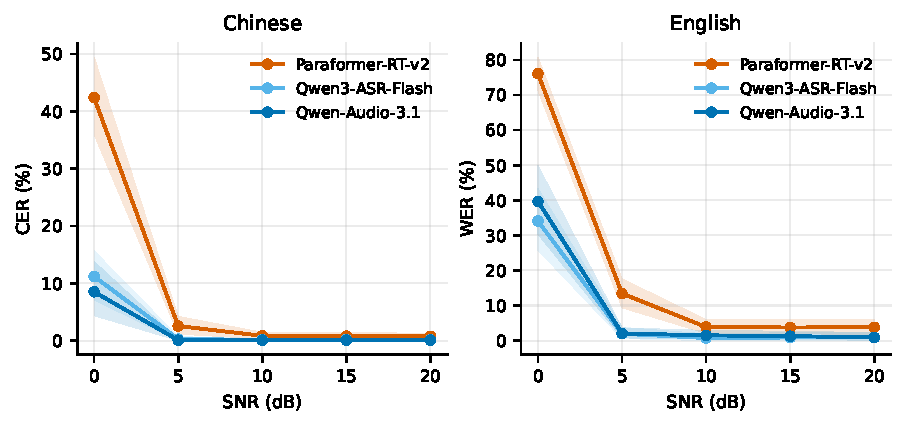
\includegraphics[width=\textwidth]{../figures/fig3_snr_curves.pdf}
\caption{Recognition error rate against babble noise signal-to-noise ratio
for four systems and both languages, with bootstrap 95 percent confidence
bands, on the 144-sentence severity sweep (72 sentences per language per
point). Dashed horizontal line marks the ten percent error level used for
the knee thresholds of Table~\ref{tab:slopes}.}
\label{fig:snr}
\end{figure}

\begin{table}[t]
\centering
\caption{Noise severity characteristics on the eight-level sweep: the
signal-to-noise ratio at which the piecewise-linear interpolation of the
measured curve crosses ten percent error, with sentence-level bootstrap 95
percent confidence intervals; the maximum slope of the fitted logistic as
a knee-sharpness measure (the fitted knee of both LLM-ASR systems in
Mandarin lies between 0 and $-5$~dB, where no observation level exists);
the steepest observed segment slope between adjacent measured levels; and
sub-range OLS slopes, listed for continuity with common practice and
depending strongly on the fitted range.}
\label{tab:slopes}
\footnotesize
\setlength{\tabcolsep}{1.8pt}
\begin{tabular}{lcccccccc}
\toprule
 & \multicolumn{2}{c}{SNR@10\% (dB)} & \multicolumn{2}{c}{Max slope} & \multicolumn{2}{c}{Steep.\ seg.} & \multicolumn{2}{c}{OLS 20--0} \\
System & zh & en & \multicolumn{2}{c}{(pp/dB)} & \multicolumn{2}{c}{(pp/dB)} & \multicolumn{2}{c}{(pp/dB)} \\
\midrule
Paraformer-RT-v2 & 2.5 (2.3,3.3) & 6.8 (5.0,7.9) & 20.8 & 16.1 & 13.0 & 15.2 & $-1.44$ & $-2.97$ \\
Paraformer-RT-8K & 8.8 (8.2,9.4) & n/a & 10.4 & n/a & 9.9 & n/a & $-3.31$ & n/a \\
Qwen-Audio-3.1 & $-0.1$ ($-0.2,0.6$) & 2.4 (2.1,3.4) & 35.5 & 21.3 & 23.7 & 12.6 & $-0.26$ & $-1.31$ \\
Qwen3-ASR & 0.3 ($-0.1,1.0$) & 2.0 (1.7,2.3) & 25.2 & 25.0 & 18.7 & 13.5 & $-0.35$ & $-1.06$ \\
\bottomrule
\end{tabular}
\end{table}

\subsection{Validation on real recorded speech}
\label{sec:results:real}

The real-speech protocol of Section~\ref{sec:methods:real} replicates the
central regularities of the synthetic pipeline while calibrating two of
its absolute levels. On clean real recordings all four systems remain
usable, with error rates of 0.8--1.2\% for the audio-LLM systems, 3.6--4.1\%
for the 16~kHz streaming specialist, and 5.1\% for the telephone-band
specialist; these are within a few points of their synthetic clean floors,
confirming that near-clean performance measured on synthetic speech
transfers to human recordings of read speech. Real-room reverberation at
matched $T_{60}$ proves markedly milder than the synthetic exponentially
decaying response: LLM error rates remain at 1.2--1.6\%, and the
telephone-band specialist, which loses 18.2\% CER under the synthetic
response, loses just 6.3\% under real rooms. The explanation is acoustic:
the synthetic response's direct-to-reverberant ratio of $-27.6$~dB is far
below the survey median of $+7.3$~dB for everyday spaces at conversation
distance, so the synthetic condition is best read as a stress case at the
reverberant extreme rather than a typical room.

Real multi-talker babble reproduces the knee-and-collapse structure of
Fig.~\ref{fig:snr} with a harder noise floor
(Fig.~\ref{fig:realval}). At $+5$~dB the audio-LLM systems already sit at
4.7--15.0\% Mandarin CER where synthetic babble left them below 0.3\%, and
at $0$~dB the gap widens to 46.9\% (Qwen-Audio) and 117.5\% (Qwen3-ASR)
against 8.5--11.2\% under synthetic babble, consistent with real babble
being less stationary and more confusable with the target than TTS-derived
interference. The real-speech data also bound the class-level
noise-tolerance claim, and the bound is worth stating precisely. The
audio-LLM advantage is real but confined to the near-knee regime: at
$+5$~dB both LLM systems err less than either streaming specialist
(4.7 and 15.0 against 40.1 and 48.6\% Mandarin CER), and Qwen-Audio
continues to hold an advantage at 0~dB (46.9 against 102.6\%), crossing
ten percent Mandarin error at 4.4~dB while both streaming specialists
exceed ten percent already at $+5$~dB, the highest SNR tested. Qwen3-ASR,
by contrast, already exceeds the ten percent level at $+5$~dB (15.0\%),
crosses at a level comparable to the specialists, and in the hallucination
regime the ordering inverts: at $-5$~dB its Mandarin CER of 207.6\% is
worse than the 16~kHz specialist's 164.4\%, and at 0~dB its 117.5\% is
worse than 102.6\%. In English the inversion appears earlier: at $-5$~dB
Qwen-Audio (86.6\%) and the specialist (86.1\%) are statistically
indistinguishable. The correct summary is therefore not that the LLM
class advantage widens under real babble, but that it holds in the
near-knee and low-error regime and disappears, for one of the two LLM
systems outright reverses, once error rates pass the ten-percent level
into the hallucination regime. The three-SNR design (75 sentences per
cell) interpolates the crossing levels rather than measuring them
directly, so the crossings themselves carry the same interpolation caveat
as the synthetic knees.

The $-5$~dB hallucination regime replicates and sharpens the synthetic
finding, and the error-type decomposition locates it precisely. Mean
Mandarin CER exceeds 100\% for every system (150.0\% for Qwen-Audio,
207.6\% for Qwen3-ASR, 164.4\% for the 16~kHz specialist), 53--79\% of
LLM utterances exceed 100\% CER individually, and the Qwen-Audio refusal
rate rises to 29.3\% (Mandarin) and 18.7\% (English), closely matching
the synthetic-condition refusal behaviour. Decomposing the alignment
errors shows that the insertion dominance is a Mandarin phenomenon: at
$-5$~dB real babble, insertions account for 45\% of Qwen-Audio's and
56\% of Qwen3-ASR's Mandarin error mass against 1.6\% for the telephone
specialist, whereas in English every system is deletion-dominated
(insertion fractions 0.9 to 12.4\%), consistent with the synthetic
sub-zero pattern where the LLM systems' Mandarin insertion fractions reach
29--34\% but their English fractions stay below 6\%. Real non-speech
transport noise at 0~dB is degradative but far gentler than real babble
(10.9\% CER for Qwen-Audio against 46.9\%), confirming that
speech-shaped interference is the harder stressor for these systems
regardless of whether the babble is synthetic or recorded.

The cascade conclusions also transfer, with one scoring caveat that the
validation design itself surfaces. Cascade BLEU on real speech falls
monotonically from 69.2/68.9 (Mandarin/English, clean) through 63.7/68.6
at $+5$~dB and 43.7/47.8 at $0$~dB to 6.9/7.6 at $-5$~dB, and regressing
BLEU loss on recognition error rate across the six conditions gives an
empirical pass-through of 0.41 (Mandarin, condition-level bootstrap 95\%
CI 0.39 to 0.67) and 0.73 (English, CI 0.60 to 0.91) with $r = 0.994$ and
0.998, bracketing the synthetic-grid values; the direction difference
between the two slopes is itself part of the finding, and the
condition-level intervals, not the sentence-level ones, are the honest
uncertainty of a relation fitted over six operating points. The
end-to-end comparison, by contrast, must be read through the reference
lens established in Section~\ref{sec:results:dual}: the validation
reference is the cascade's own engine applied to human transcripts, so it
is same-engine with the cascade and foreign to LiveTranslate, and the
absolute gap of 27 to 28 BLEU on clean speech (69.1 against 42.0) is
therefore not a translation-quality measurement. Two observations
nevertheless survive any reference choice. First, the mechanism of the
bias is visible directly: on clean real speech the cascade's ASR frontend
reproduces the human transcript exactly on 133 of 150 sentences, and the
engine reproduces its own reference exactly (self-BLEU 100), so the
cascade's 31-point distance from the reference on the remaining 17
sentences shows how strongly the engine's word choice responds to
punctuation and inverse-text-normalisation differences in its input,
which BLEU then penalises at full weight. Second, the within-path
relative losses are reference-invariant, and there the end-to-end path is
the more fragile one: from clean to 0~dB real babble, LiveTranslate loses
41.6 percent of its own clean BLEU against 33.7 percent for the cascade.
The conclusion that end-to-end paths are not automatically more robust is
therefore confirmed on real speech in the relative-loss sense, while the
absolute BLEU ordering of the two paths on this reference is reported only
as a same-engine artefact, in line with the dual-reference analysis of
Section~\ref{sec:results:dual}.

\begin{figure}[t]
\centering
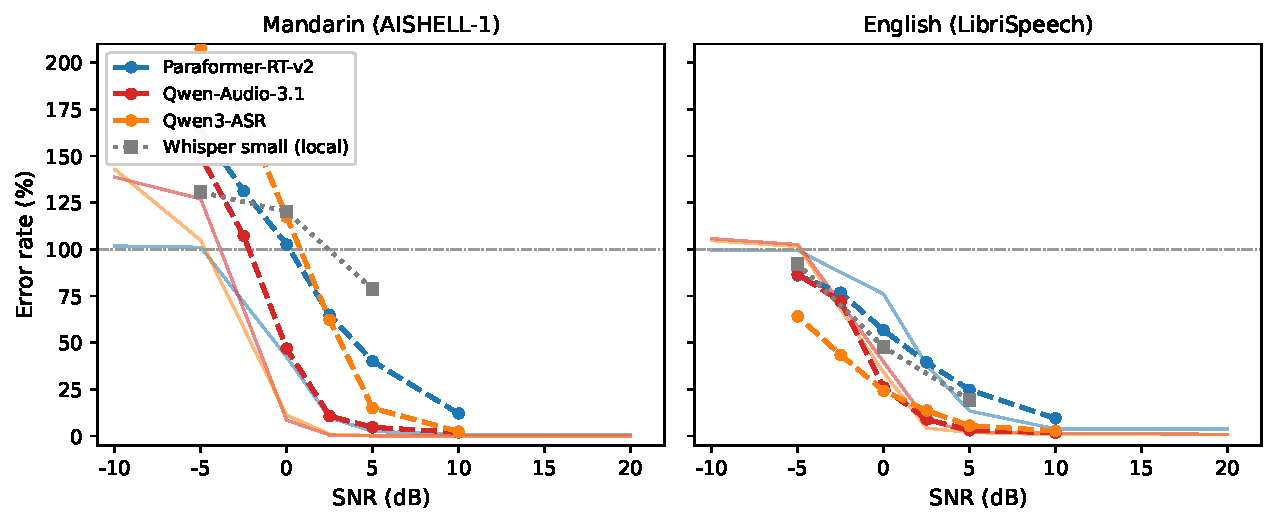
\includegraphics[width=\textwidth]{../figures/fig8_real_validation.pdf}
\caption{Recognition error rate versus SNR under synthetic babble (thin
solid lines, 8-point sweep with 95\% bootstrap bands) and real multi-talker
babble (thick dashed lines with markers, three SNRs) on real recorded
speech. Left: Mandarin (AISHELL-1 test); right: English (LibriSpeech
test-clean). Real babble is the harder stressor at every SNR, but the
system ordering, the knee structure, and the sub-0~dB hallucination regime
(CER above 100\%, dotted line) all replicate.}
\label{fig:realval}
\end{figure}

\subsection{Cascade versus end-to-end translation under degradation}
\label{sec:results:cascade}

Fig.~\ref{fig:cascade} compares the speech translation paths across the
main grid, and Table~\ref{tab:translation} reports the corresponding scores
with both references, bootstrap confidence intervals, sample sizes, and
the refusal-inclusive chrF. On
clean audio the three cascades lose almost nothing relative to their
translation oracle, the text translation engine applied to perfect
transcripts, which scores 55.5 BLEU against the primary reference. The
cascade built on Qwen-Audio 3.1 starts at 53.9 BLEU ($n{=}144$), the
cascade built on the streaming specialist at 51.5, the cascade built on
Qwen3-ASR at 53.2, and the end-to-end omni path scores highest at 68.1
($n{=}84$) with the streaming LiveTranslate service at 59.8 ($n{=}144$).
Under degradation the ordering and the magnitudes change dramatically. At
0~dB the Qwen-Audio cascade drops 9.8 BLEU points, the streaming-specialist
cascade collapses by 35.7 points to 15.8 BLEU, the Qwen3-ASR cascade drops
10.2 to 43.0, the omni end-to-end path loses 22.5 points, and the streaming
translation service loses 9.3 points from a lower starting level. The
sentence-level confidence intervals of Table~\ref{tab:translation} are
wide relative to these movements, so the 0~dB collapses are unambiguous
while adjacent-system differences of one to two points are not. The
refusal-inclusive chrF tells the same story with the empty outputs counted:
the Qwen-Audio cascade falls from 65.2 to 53.7 chrF at 0~dB once its eight
refused sweep sentences are scored as empty translations, a drop that
corpus BLEU would understate because its brevity penalty saturates when
hypotheses are longer than references, which is why both metrics are
reported.

\begin{figure}[t]
\centering
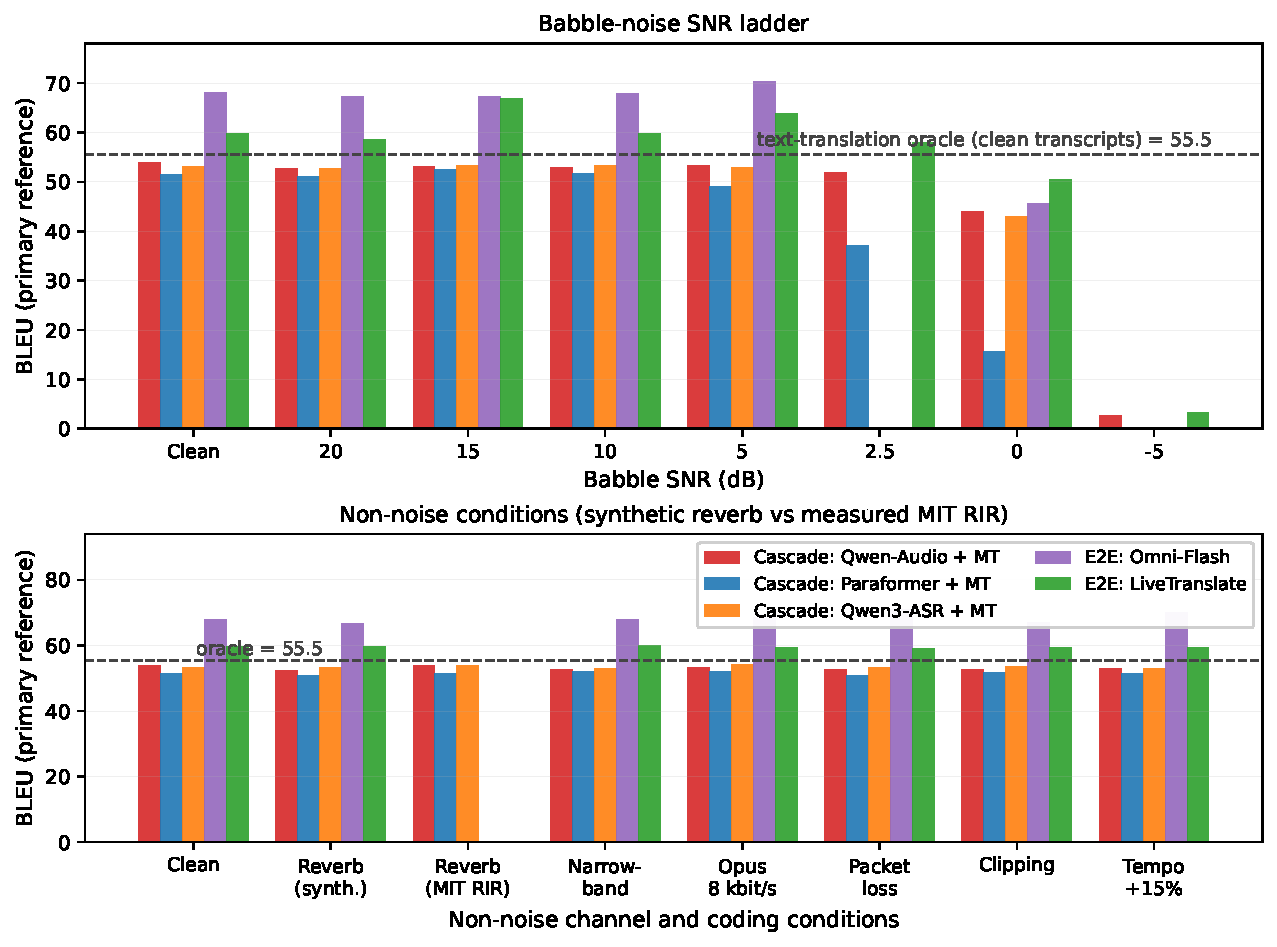
\includegraphics[width=\textwidth]{../figures/fig4_cascade_e2e.pdf}
\caption{Translation quality of the two best cascades and the two
end-to-end speech translation paths across the main degradation grid,
scored against the same-vendor LLM reference
(Section~\ref{sec:results:dual}); the third cascade (Qwen3-ASR frontend)
tracks the Qwen-Audio cascade within 1.1 BLEU points throughout and is
tabulated in Table~\ref{tab:translation} instead of plotted. The hatched
bar is the text-translation oracle on
clean transcripts.}
\label{fig:cascade}
\end{figure}

\begin{table}[t]
\centering
\caption{Translation quality by condition: macro-averaged BLEU against the
primary reference (Qwen3.8-Max translations of clean transcripts) with
sentence-level bootstrap 95\% confidence intervals, the score against the
secondary reference (oracle cascade output), the clean-to-0~dB
relative loss, refusal-inclusive chrF, and per-cell $n$. Cascade scores at
0~dB are conditional on a non-empty frontend output; the refusal-inclusive
chrF counts refused sentences as empty translations. The omni path is
scored on its quota-limited subset and is compared with the other paths on
the common subset in the text.}
\label{tab:translation}
\footnotesize
\setlength{\tabcolsep}{1.6pt}
\begin{tabular}{lcccccc}
\toprule
 & & \multicolumn{3}{c}{Babble 0 dB} & & \\
System & Clean & BLEU (95\% CI) & vs & rel. & chrF & chrF \\
 & BLEU & & oracle & loss & 0~dB & clean \\
\midrule
Oracle MT (clean text) & 55.5 & -- & -- & -- & -- & 66.7 \\
Cascade: Paraformer+MT & 51.5 & 15.8 & 17.4 & 69\% & 26.9 & 63.4 \\
 & (47.7,55.6) & (12.3,19.1) & & & & \\
Cascade: Qwen-Audio+MT & 53.9 & 44.1 & 68.3 & 18\% & 53.7 & 65.0 \\
 & (50.4,57.8) & (40.1,48.3) & & & & \\
Cascade: Qwen3-ASR+MT & 53.2 & 43.0 & 66.7 & 19\% & 53.4 & 65.4 \\
 & (49.4,57.1) & (38.7,47.9) & & & & \\
E2E: Omni-Flash & 68.1 & 45.5 & 34.4 & 33\% & 51.6 & 73.0 \\
 & (61.3,74.6) & (38.2,50.5) & & & & \\
E2E: LiveTranslate & 59.8 & 50.4 & 44.9 & 16\% & 56.2 & 68.5 \\
 & (56.2,63.2) & (41.8,51.4) & & & & \\
\bottomrule
\multicolumn{7}{l}{\footnotesize $n$: cascades 144 clean, 135--144 non-empty at 0~dB; omni 84; LiveTranslate 144/132;}\\
\multicolumn{7}{l}{\footnotesize CIs from 300 sentence-bootstrap resamples.}
\end{tabular}
\end{table}

Three conclusions follow. The first concerns the frontend hypothesis. The
translation quality of a cascade under acoustic degradation is governed
largely by the robustness of its recognition stage: swapping the
frontend from the streaming specialist to the LLM recogniser at 0~dB is
worth 28 BLEU points (44.1 against 15.8) on the same backend, and the third cascade, built on
Qwen3-ASR, tracks the Qwen-Audio cascade within 1.1 BLEU points (mean gap
0.5, maximum at 0~dB) across the twelve
shared conditions, which shows that the pattern generalises across
frontends of the same class. What the present design cannot separate is the
contribution of the translation engine, since every cascade shares one
backend; the frontend comparison is within-backend and valid, but a claim
that the frontend dominates the choice of engine would require varying the
engine too. The second qualifies the common expectation that end-to-end
systems avoid cascade error propagation and are therefore more robust. At
0~dB the omni end-to-end path loses a third of its BLEU score, more than
the well-frontended cascades lose at 18 and 19 percent. Its apparent
absolute lead over the cascades is, however, an artefact of two
confounds: its clean score of 68.1 is measured on a quota-limited subset
of 84 sentences and carries reference affinity
(Section~\ref{sec:results:dual}), and on the sentences common to both
paths the 0~dB picture reverses, with the Qwen-Audio cascade at 47.1
against omni 45.5, a paired difference whose bootstrap interval ($-11.3$
to $+5.5$) spans zero. The defensible statement is therefore about
degradation behaviour, not absolute ranking: the omni path degrades more
than the well-frontended cascades at 0~dB. The streaming
LiveTranslate service is the most degradation-resilient of the paths,
losing 16 percent at 0~dB, which is consistent with the behaviour of its
internal frontend recogniser documented in
Section~\ref{sec:results:frontend}. End-to-end designs do not inherit
robustness automatically; they inherit the robustness of whatever acoustic
frontend their provider trained internally, which in this measurement is
better than the specialised streaming ASR but not automatically better
than the best cascade.

The condition-wise structure of Fig.~\ref{fig:cascade} adds three nuances to
this picture. First, apart from the 0~dB point the cascade built on the LLM
recogniser is essentially flat across the entire grid, moving within one
BLEU point of its clean score under every other condition, which mirrors the
recognition flatness of Table~\ref{tab:main} and confirms that the
non-noise degradations are, at deployed severities, engineering noise rather
than failure modes for a robust frontend. Second, the streaming translation
service shows the same flatness with a single exception: its narrowband
score of 60.1 sits marginally above its clean score, and its packet-loss and
tempo scores are likewise within half a point of clean, so its 0~dB loss is
the only substantive degradation it suffers. Third, the omni end-to-end path
exhibits a small but consistent anomaly: its packet-loss and tempo scores,
at 71.1 and 70.0, exceed its clean score of 68.1. Inspection of the outputs
suggests that under these mild distortions the model produces slightly more
concise translations that happen to align better with the reference style,
rather than genuinely better translations; the effect is within the
reference-sensitivity margin documented in Section~\ref{sec:results:dual}
and is a further argument for treating small absolute differences between
heterogeneous systems with caution.

Decomposing the 0~dB collapse by direction sharpens the frontend story. The
specialist cascade loses 25.9 BLEU points in the Chinese-to-English
direction but 45.6 points in the English-to-Chinese direction, falling to
8.7 BLEU, because its English recognition, at 75.5 percent error, destroys
the source representation before the translation stage operates. The
LLM-frontend cascade degrades far less but still asymmetrically, losing 4.7
points in the Chinese-to-English direction and 15.0 in the other, a 3.2 to
one ratio, and the omni path shows the same skew at 19.4 against 25.7. The
streaming translation service loses almost nothing in the
Chinese-to-English direction at 0~dB, at 56.0 against 57.3 clean, but 18.3
points in the other direction, which parallels the language asymmetry of
its internal frontend. No path degrades symmetrically, so direction-symmetric
deployment claims should be checked per direction rather than
pooled.

\subsection{Reference sensitivity of translation scoring}
\label{sec:results:dual}

Table~\ref{tab:translation} also reports scores against the secondary
reference, the oracle cascade output. The two references invert the apparent
ordering of the systems on clean audio. Against the primary reference,
produced by the provider's strongest text LLM, the omni end-to-end path
leads at 68.1 BLEU, exceeding even the text-translation oracle at 55.5.
Against the oracle reference the same end-to-end path scores 48.5 while the
Qwen-Audio cascade scores 89.6, since the cascade shares its translation
engine with the reference generator. The inversion repeats at 0~dB: the
omni path leads the Qwen-Audio cascade by 1.4 points against the primary
reference but trails it by 33.9 points against the oracle reference. The
inversion quantifies a hazard for any evaluation that scores machine
translation against machine-generated references, and it is sharpened here
by the fact that all systems and both reference generators come from one
vendor, so no reference in this study is family-disjoint from every system
under test; the primary reference at least comes from a different product
line than any translation path. Two safeguards make the present conclusions
robust to this effect. Degradation losses are computed within a system
against a fixed reference, so the percentage losses reported above do not
depend on the choice, and the ordering of relative losses at 0~dB, at 69,
33, 19, 18, and 16 percent, is preserved under both references. We
recommend that future black-box translation evaluations score against at
least two references generated by different model families from each other
and from every system under test, state the family relationships
explicitly, and treat cross-family absolute comparisons as provisional
until human-reference anchored.

\subsection{Error pass-through from recognition to translation}
\label{sec:results:cac}

Fig.~\ref{fig:cac} relates the BLEU loss of the three cascades to their mean
recognition error rate across all operating conditions, fifteen per
cascade for the two original frontends and twelve for the Qwen3-ASR cascade,
spanning recognition error rates from 0.3 to over 100 percent. The error
metric on the horizontal axis is the sweep-subset mean recognition error
with refusals counted as complete failures, matching the protocol of
Table~\ref{tab:main}, and the vertical axis is the BLEU loss from each
cascade's clean score against the primary reference. The relationship is
strongly linear across this range: the Pearson correlation is 1.00 for the
Qwen-Audio cascade, 0.995 for the specialist cascade, and 0.994 for the
Qwen3-ASR cascade. Three cautions, however, separate this empirical
relation from a law, and each is quantified rather than asserted. First,
the correlation is concentrated in a few high-error conditions: the points
cluster near the origin for the nine mild conditions, so the line is
anchored chiefly by the four to five collapsed conditions, which is why
leave-one-condition-out refits are stable for the first two cascades
(slopes move by less than 0.03) but not for the third, where dropping the
0~dB condition moves the Qwen3-ASR slope from 0.47 to 0.74. Second, the
sentence-level bootstrap intervals understate the design uncertainty:
resampling the operating conditions themselves gives 95 percent intervals
of 0.23 to 0.45 for the Qwen-Audio cascade, 0.52 to 0.66 for the
specialist cascade, and 0.38 to 3.9 (heavily right-tailed, median 0.47)
for the Qwen3-ASR cascade, so the condition mix, not the sentence sample,
is the dominant source of uncertainty in the slope. Third, the slope is
not constant across the error range: excluding the conditions above 40
percent recognition error moves the slope from 0.44 to 0.37 for the
Qwen-Audio cascade and from 0.54 to 0.68 for the specialist cascade, and
the linear form cannot hold without bound on the high side, because BLEU
loss saturates at the clean score while recognition error can exceed 100
percent through insertions. Within these bounds the fitted relation, with
explicit intercepts of $+0.6$ and $-1.0$ BLEU points (both statistically
indistinguishable from zero, and small enough that the through-origin
reading changes no prediction by more than a point), gives slopes of 0.44
BLEU points per percentage point of recognition error for the Qwen-Audio
cascade (sentence-level bootstrap 95\% CI 0.41 to 0.48), 0.54 for the
specialist cascade (0.51 to 0.58), and 0.47 for the Qwen3-ASR cascade
(0.35 to 0.60). The
steeper slope for the specialised frontend reflects the composition of its
errors under severe noise, which include whole-utterance failures where the
translation engine receives little or no usable signal, whereas the LLM
recogniser's residual errors under moderate degradation are concentrated in
individual words that the translation engine can often route around. A
service integrator can therefore use the rule as an empirical rule of
thumb, valid for error rates up to roughly 60 percent and for this
translation engine:
every percentage point of recognition error costs roughly half a BLEU point
downstream, with the caveat that the cost drifts toward two thirds of a
point for error profiles dominated by whole-utterance failures and toward
two fifths for error profiles dominated by isolated word errors, that the
honest uncertainty of the coefficient is the condition-level interval
rather than the sentence-level one, and that
the estimate is calibrated on one translation engine and should be
re-estimated if the backend changes.

\begin{figure}[t]
\centering
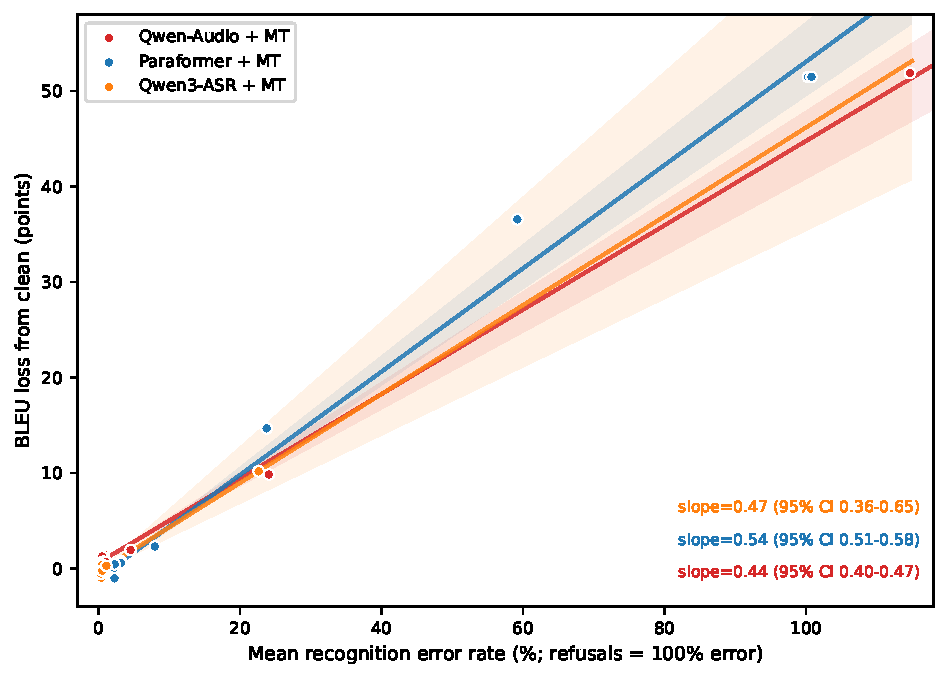
\includegraphics[width=0.6\textwidth]{../figures/fig6_cac.pdf}
\caption{Translation quality loss against mean recognition error rate
for three cascades over fifteen operating conditions for the two original
frontends and twelve for the Qwen3-ASR frontend, with fitted linear
pass-through (with intercept) and 95\% confidence bands. Recognition error
is the sweep-subset mean with refusals counted as complete failures;
sub-zero-dB conditions extend the range beyond 100 percent through
insertion errors. Mild conditions cluster near the origin; the fit is
anchored chiefly by the collapsed conditions.}
\label{fig:cac}
\end{figure}

\subsection{The streaming translation frontend as a recogniser}
\label{sec:results:frontend}

The streaming translation service exposes its internal recognition output,
which allows its frontend, a specialised streaming recogniser, to be scored
as a sixth system on the same 144-sentence sweep subset as the directly
purchasable systems, which is the comparison reported here. Its
clean-condition error rate of 1.0 percent sits between the LLM-ASR systems
at 0.4 and the general-purpose streaming specialist at 2.2 percent, a
difference that is not individually significant, and
under noise it tracks the LLM-ASR class rather than its own product class:
at 0~dB it errs at 25.4 percent against 24.1 and 22.6 percent for the two
LLM-ASR systems, with overlapping confidence intervals and no significant
paired difference (Wilcoxon $p=0.19$), while the general-purpose streaming
specialist errs at 59.2 percent on the same sentences. At 2.5~dB it errs at
4.0 percent against 4.5 and 2.6 for the LLM systems. Two coverage caveats
apply: the frontend is only observable where the translation session
completed, so its sweep coverage is partial in some conditions (52 to 134 of
144), and its zero-error 5~dB figure in the appendix rests on 52 completed
sessions and should not be read as outperforming its own clean score. The
observation remains noteworthy for practitioners: a recogniser competitive
with the best purchasable ASR of this provider under severe noise is not
available as a recognition service but is embedded inside a translation
product, which suggests that providers optimise internal streaming
frontends for exactly the acoustic conditions where end-to-end translation
must survive.

\subsection{Sentence-level variability and latency}
\label{sec:results:latency}

Fig.~\ref{fig:dist} shows the sentence-level error distributions for the
strongest LLM recogniser and the specialised streaming recogniser on five
representative conditions. The distributions are strongly right-skewed:
under moderate degradation most sentences remain nearly correct while a
tail of sentences fails completely, which is why the confidence intervals in
Table~\ref{tab:main} are wide relative to their means. Under 0~dB babble the
median sentence is still recognised reasonably well by the LLM systems while
the upper quartile fails outright, a heterogeneity that aggregate error
rates conceal and that matters for applications with per-utterance quality
requirements. The skew also explains a statistical property visible
throughout Table~\ref{tab:main}: the confidence intervals of the LLM systems
under moderate degradation are wide relative to their means because a small
number of complete failures, including the refusal cases, coexist with a
large mass of near-perfect transcripts. For a system operator this shape
matters more than the mean, since the tail sentences are the ones that
generate complaints and downstream errors, and the fraction of sentences
above a given error threshold is a more actionable deployment metric than
the average. On the 0~dB condition, the fraction of English sentences with
error rates above 50 percent is 83 percent for the specialised streaming
recogniser against 36 percent for Qwen3-ASR, while in Chinese the same
threshold is exceeded by 33 percent of sentences for the specialised system
against 3 percent for Qwen-Audio, so the family gap in tail behaviour is
considerably larger than the gap in means.

\begin{figure}[t]
\centering
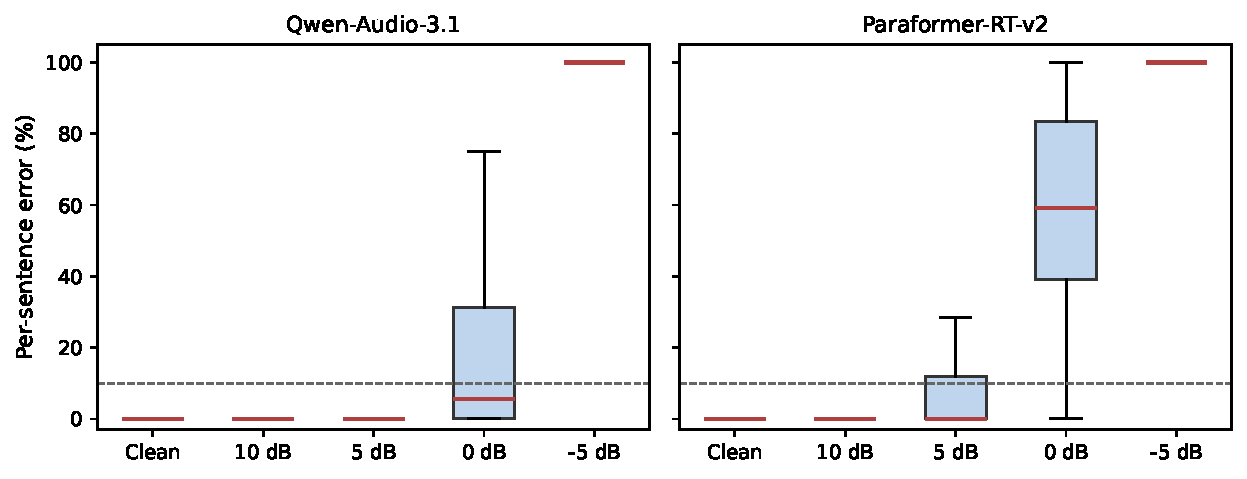
\includegraphics[width=\textwidth]{../figures/fig5_distribution.pdf}
\caption{Sentence-level error distributions by condition for the strongest
LLM recogniser and the specialised streaming recogniser.}
\label{fig:dist}
\end{figure}

Table~\ref{tab:latency} reports whole-utterance turnaround latencies. The
text translation stage, benchmarked separately with 120 sequential timed
calls, completes in 0.35 seconds per sentence on average (median 0.26, 95th
percentile 0.46), so the fastest cascade that this provider can assemble,
Qwen3-ASR feeding the translation engine, completes in about 0.7 seconds
per sentence on average, the Qwen-Audio cascade in about 1.2 seconds, and
the omni end-to-end path averages 2.8 seconds with a 95th percentile above
7 seconds, reflecting the substantially longer generation path of an
omni-modal foundation model that produces its translation in a single
response. The streaming translation service completes in about half a
second per utterance. These figures are whole-utterance turnaround, not
first-partial latency: the streaming interfaces would show substantially
lower time-to-first-text than the whole-utterance numbers suggest, so
latency comparisons across interface classes should be treated as
indicative. Latency therefore reinforces rather than reverses the accuracy
picture: the paths that degrade least under noise, the well-frontended
cascades and the streaming translation service, are also among the fastest,
while the slowest path, the omni end-to-end model, is the most fragile
under severe noise in this measurement.

\begin{table}[t]
\centering
\caption{Whole-utterance API turnaround latency in seconds for the
recognition systems, the text translation stage (120 sequential timed
calls), and the end-to-end paths. Streaming interfaces are measured at
maximum feed rate; see text for the first-partial caveat.}
\label{tab:latency}
\small
\begin{tabular}{lccc}
\toprule
System & Mean & P50 & P95 \\
\midrule
Qwen3-ASR-Flash & 0.37 & 0.35 & 0.46 \\
Paraformer-RT-8K-v2 & 0.45 & 0.43 & 0.75 \\
LiveTranslate (E2E, streaming) & 0.55 & 0.52 & 0.80 \\
Qwen-Audio-3.1-Flash & 0.80 & 0.72 & 1.93 \\
Paraformer-RT-v2 & 0.87 & 0.85 & 1.65 \\
Text translation (qwen-mt-uni, $n{=}120$) & 0.35 & 0.26 & 0.46 \\
Qwen3.8-Omni-Flash (E2E) & 2.77 & 2.20 & 7.19 \\
\bottomrule
\end{tabular}
\end{table}

The repetition runs quantify how much of the measured variation is
run-to-run noise rather than signal. Re-running the two LLM-ASR systems
twice on the 0~dB babble and tempo conditions yields condition-level error
rates that vary by at most 0.9 percentage points across three runs
(0~dB: 24.1, 24.9, and 24.4 for Qwen-Audio; 22.6, 23.4, and 23.2 for
Qwen3-ASR), while individual transcripts agree in 79 to 99 percent of
sentences between runs. Condition-level conclusions in this paper are
therefore stable against decoding nondeterminism at default settings, but
sentence-level deployments should expect one in five transcripts to differ
between identical calls at the worst condition. The omni path's small
packet-loss and tempo anomalies of Section~\ref{sec:results:cascade}, two
to three BLEU points, exceed any error-rate variation we can measure on
the systems we could re-run, but the omni system's quota was exhausted
before it could be re-tested, so its anomaly remains unexplained rather
than confirmed as genuine.

\begin{figure}[t]
\centering
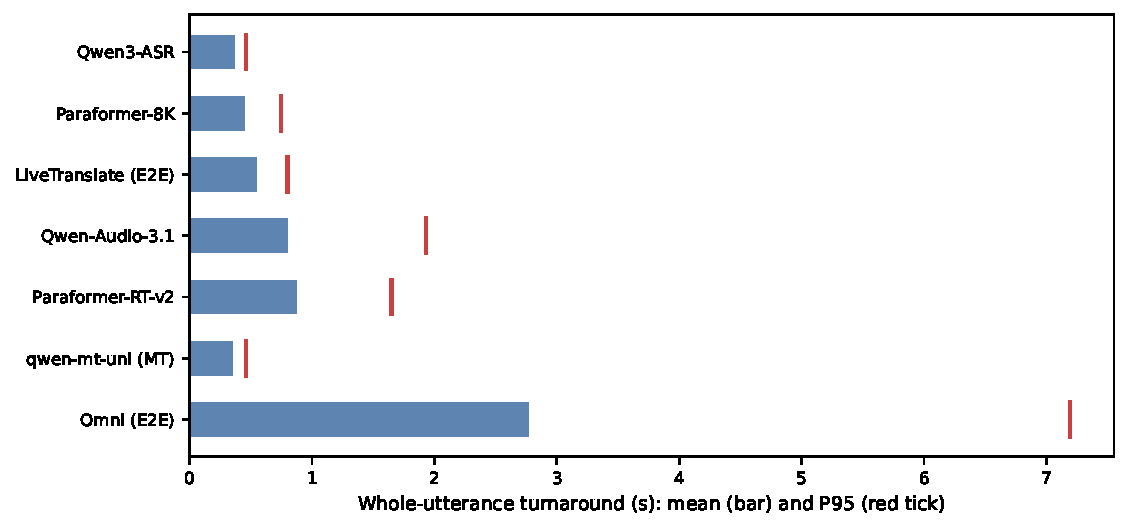
\includegraphics[width=0.5\textwidth]{../figures/fig7_latency.pdf}
\caption{API round-trip latency by system, mean and 95th percentile.}
\label{fig:latency}
\end{figure}
